\section{Materials and Methods}
\label{sec:methods}

The design of the study follows from the gaps listed in Section~\ref{subsec:gaps}. We use a multi-object detector and not a classifier (G1), apply a swarm optimizer to the training hyperparameters of this detector (G2), compare it with random search and the defaults at an equal budget using confidence intervals on a test split that is used once (G3), and keep separate studio, real-world and Indian test sets (G4).

\subsection{Experimental Design}
\label{subsec:design}

The training hyperparameters of one detector are selected by three arms, as shown in Fig.~\ref{fig:pipeline}. \armA takes the Ultralytics default values without any search and acts as the reference that tuning has to beat. \armB selects the best of 32 random samples, and \armC selects the best setting found by a swarm of 8 particles in 4 rounds. The two search arms evaluate their candidates with the same proxy training (Section~\ref{subsec:proxy}). The budget is therefore measured in proxy trainings and not in wall-clock time, since the latter varied between the methods and between cloud sessions (Section~\ref{subsec:res-cost}). The setting selected by each arm is trained once using an identical recipe (Section~\ref{subsec:training}) and evaluated once on a held-out test split (Section~\ref{subsec:eval}).

The whole experiment was performed twice. \genone is based on a single studio-style dataset with six classes and an image size of 416~px. \gentwo adds real-world training photographs, a seventh class (OTHER), an image size of 640~px and an Indian set used only for testing. The search space, PSO settings, seeds, training recipes and evaluation code are common to both generations, and both searches were run again from the beginning for \gentwo. Because the classes, image size and training data are different, the scores of the two generations cannot be treated as one benchmark. A separate comparison of the generations is described in Section~\ref{subsec:eval}.

\begin{figure}[!t]
\centering
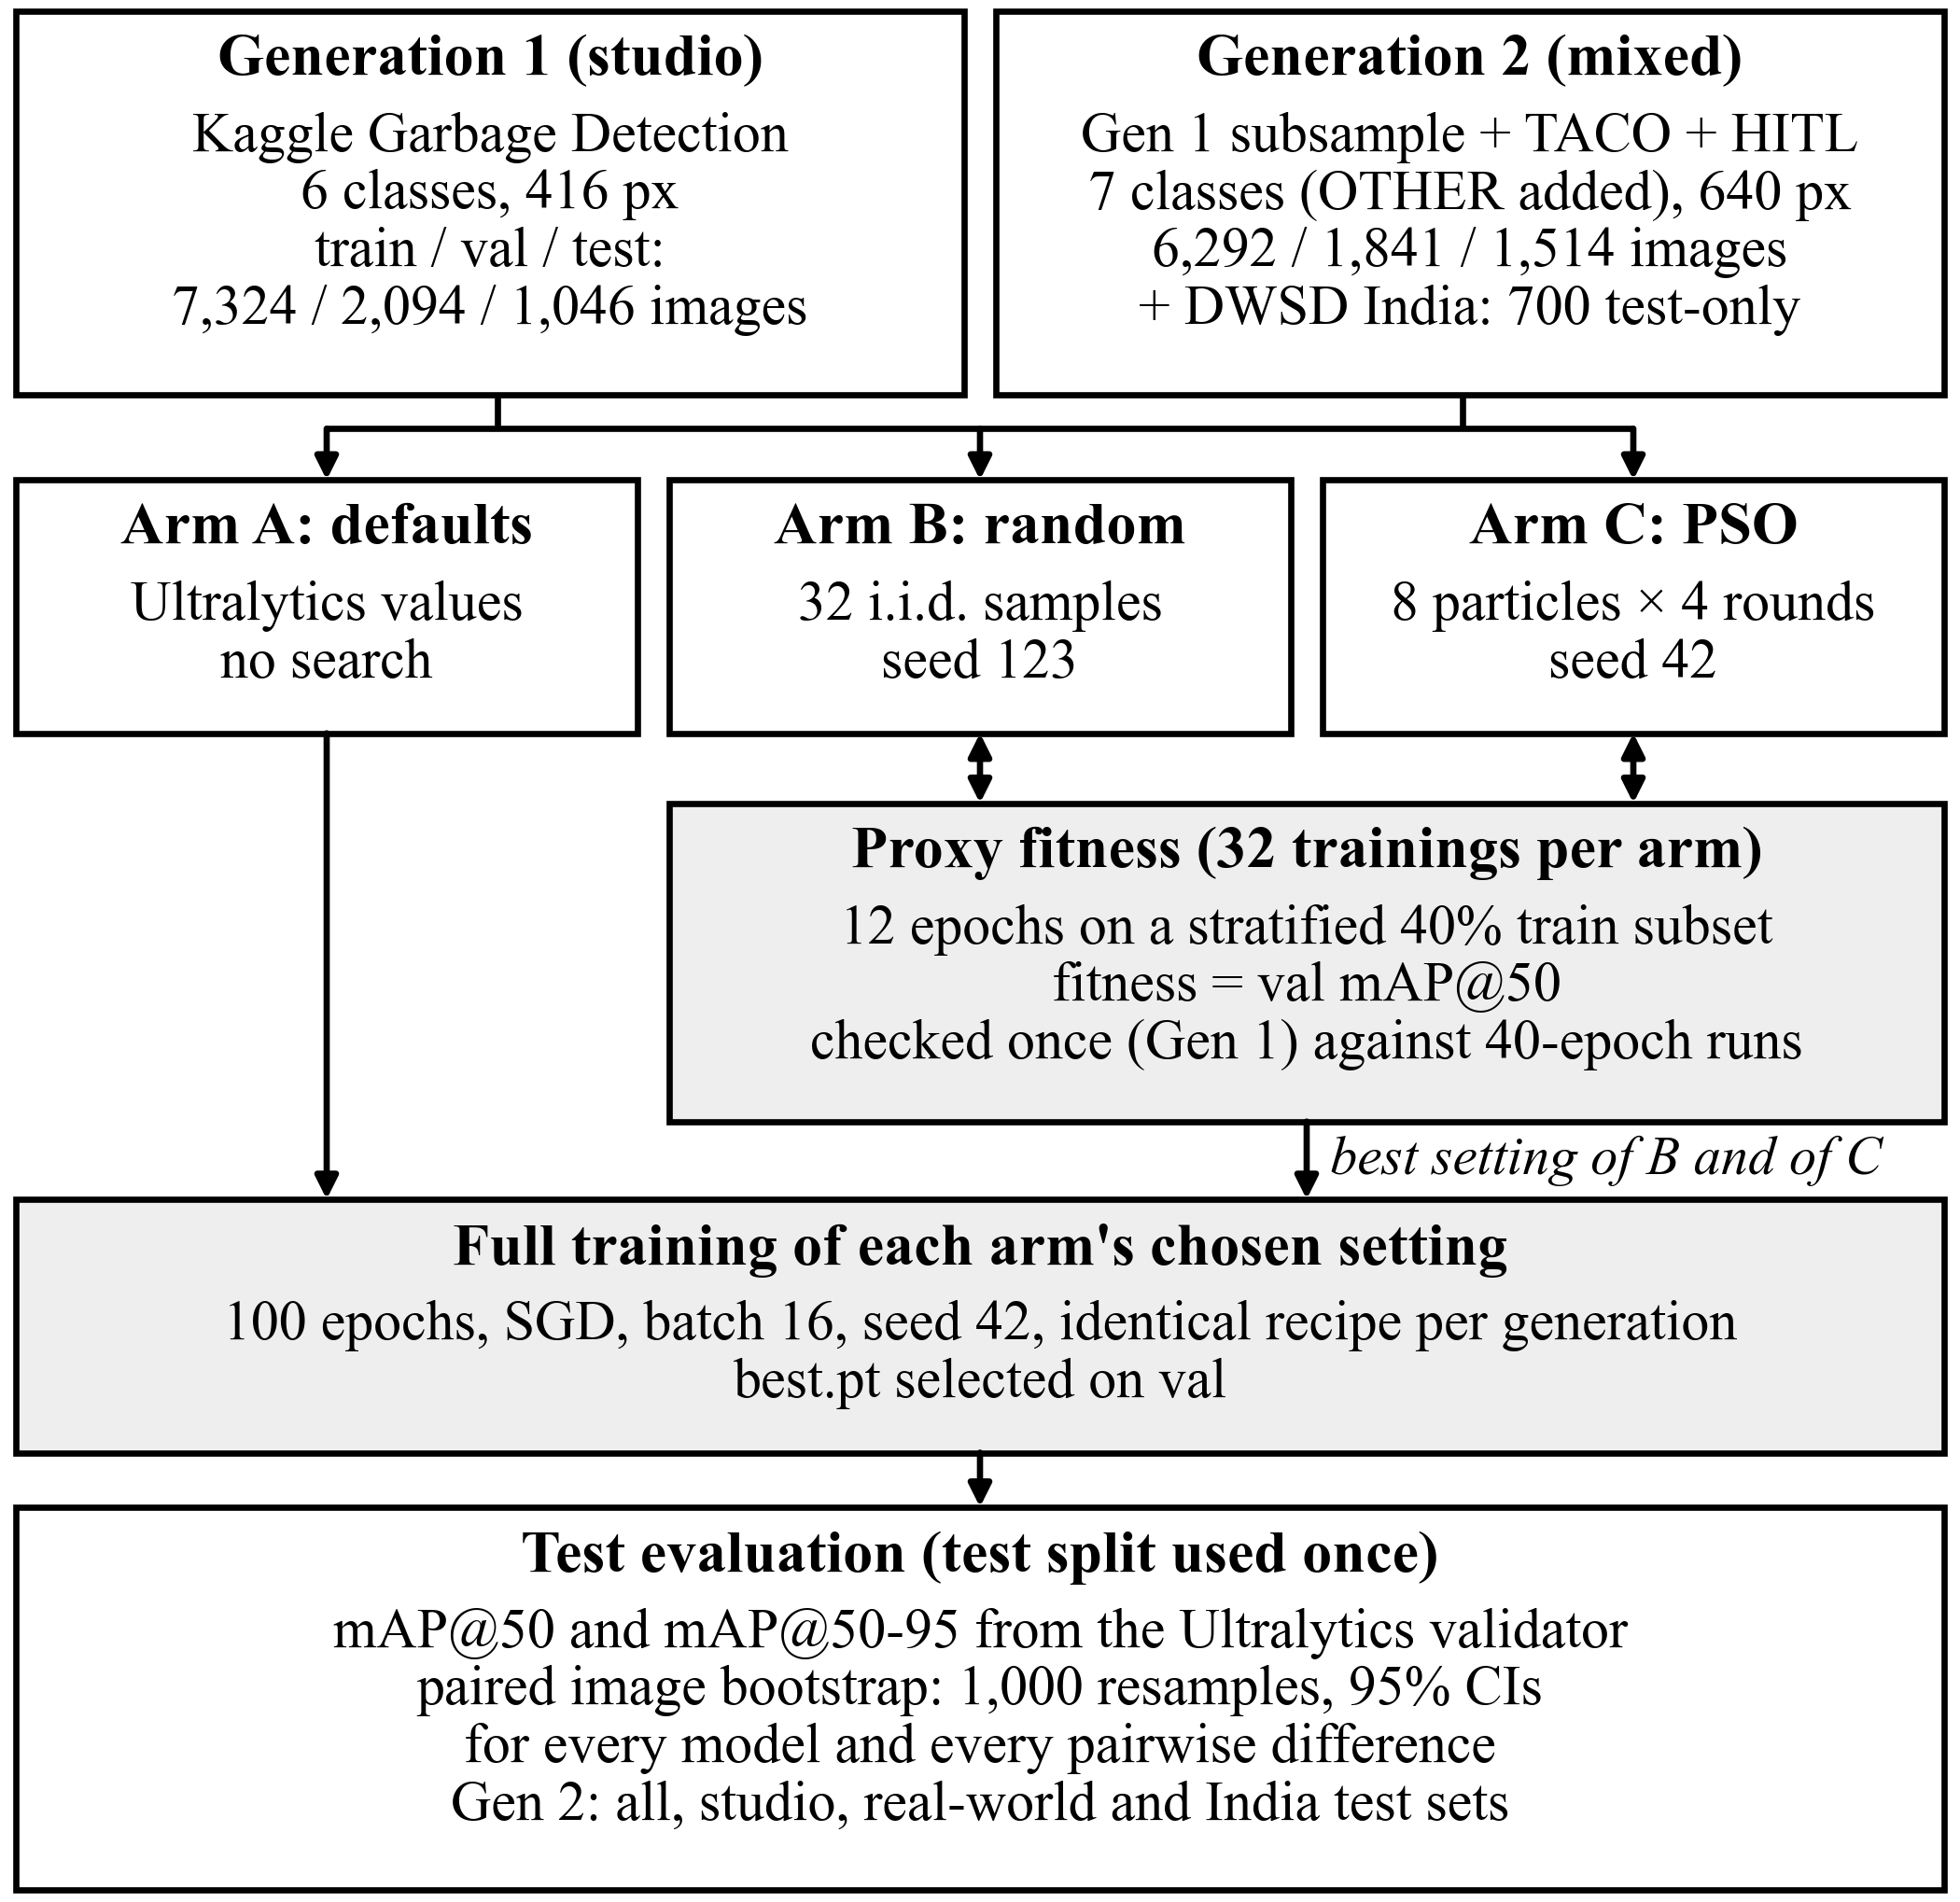
\includegraphics[width=\columnwidth]{m_pipeline.png}
\caption{Experimental pipeline used in both generations. Arms~B and~C are each allowed 32 proxy trainings, while Arm~A uses the library defaults without any search. The setting chosen by each arm is trained once for 100 epochs and tested once.}
\label{fig:pipeline}
\end{figure}

\subsection{Datasets}
\label{subsec:datasets}

All data sources are listed in Table~\ref{tab:datasets} together with their licences and split sizes.

\textit{\genone data.} We used the Kaggle dataset ``Garbage Detection -- 6 Waste Categories''~\cite{viswaprakash2024garbage}, which originates from a Roboflow project. It contains studio-style images with YOLO-format boxes for six classes: BIODEGRADABLE, CARDBOARD, GLASS, METAL, PAPER and PLASTIC. The dataset is imbalanced. In the training split, 36.45\% of the boxes occupy less than 1\% of the image area, and BIODEGRADABLE accounts for 61.92\% of the boxes whereas PAPER accounts for only 5.61\%. The folders supplied with the dataset are divided by class; the validation folder, for instance, has 13,632 BIODEGRADABLE boxes but only 33 PAPER boxes, and the test folder has no GLASS box at all. For this reason we pooled all the images and split them again in a 70/20/10 ratio, stratified by source class (seed 42), ensuring at least 30 boxes of each class in the validation and test splits. Near-duplicate images were always kept in the same split. Two images were treated as copies if their files were identical (MD5), if they came from the same Roboflow source image, if their 256-bit difference hashes differed by at most 10 bits, or if the hashes differed by at most 40 bits and the Pearson correlation between their $64\times64$ grayscale thumbnails was 0.90 or higher. In this way 47 groups comprising 133 images were found. The label checks revealed 17 zero-size boxes, and no image was corrupt or unlabeled.

\textit{\gentwo training data.} \gentwo has seven classes, i.e., the six classes of \genone with the same indices and an additional class OTHER. From the \genone splits we drew a subsample stratified by dominant class (seed 42) with 3,000 training and 900 validation images. All test images were retained, so the studio test set of \gentwo is the same as the test set of \genone. TACO~\cite{proenca2020taco} contributes crowd-sourced photographs of litter in the wild. All of its 60 categories were mapped to our classes (drink cans to METAL and cigarettes to OTHER, for example), which gave 1,260 OTHER boxes but only 8 BIODEGRADABLE boxes. The HITL Recycling dataset~\cite{hitl2026recycling} contributes street photographs, nearly all of which have a single litter box. Its objects were assigned a class from the object tag when this was decisive (food waste $\to$ BIODEGRADABLE), otherwise from the material tag (aluminum $\to$ METAL), and otherwise OTHER; 100 objects had no material tag. TACO and HITL were split 70/20/10 using the same duplicate rules, and their images were stored with the longer side limited to 640~px. The merged data contain 962 duplicate groups, and none of them extends over two sources or two splits. Within the real-world sources there are 918 byte-identical pairs. These do not cause leakage, but they give extra weight to some photographs. In the merged training set, BIODEGRADABLE has 51.96\% of the boxes and OTHER has 3.89\%. The studio images contain no OTHER box, and the real-world test set contains only one BIODEGRADABLE box.

\textit{Indian test set.} The Dense Waste Segmentation Dataset (DWSD)~\cite{ali2025dwsd} consists of 784 phone photographs of streets, parks and garbage areas in Kolkata and Berhampore, West Bengal, annotated with $448\times448$ semantic masks. This dataset was used strictly for testing and played no role in training, search or model selection. To obtain boxes, every 8-connected region of a single mask value with at least 50 pixels was converted into one box. As a consequence, items of the same class that touch each other are merged into one large box. The class mapping had to be inferred by us, because the published table of mask values does not agree with what the regions actually show (the value that is listed as background covers polythene bags in 610 masks). We assigned a name to each value after inspecting its regions, and six of the fifteen values remain uncertain. Eighty-four images that yielded no boxes were excluded since some of them show waste that is not annotated. The remaining set has 3,040 PLASTIC, 1,230 PAPER, 124 CARDBOARD, 90 OTHER and 18 METAL boxes. An MD5 comparison with the 9,647 images of the main build did not find any identical file.

\begin{table*}[!t]
\centering
\caption{Datasets. Counts are images, with boxes in parentheses. ``Classes'' is the number of target classes that occur in the source. The \gentwo studio test set equals the \genone test set; the \gentwo real-world test set is the union of the TACO and HITL test images (468 images, 779 boxes).}
\label{tab:datasets}
\footnotesize
\setlength{\tabcolsep}{4pt}
\begin{tabular}{@{}llllllccc@{}}
\toprule
Generation & Source & Domain & Licence & Stored size & Classes & Train & Validation & Test \\
\midrule
\genone & Garbage Detection (Kaggle) & studio & CC BY 4.0 & $416\times416$ & 6 & 7,324 (51,756) & 2,094 (14,904) & 1,046 (7,413) \\
\midrule
\multirow{5}{*}{\gentwo} & \genone subsample & studio & CC BY 4.0 & $416\times416$ & 6 & 3,000 (22,206) & 900 (6,904) & 1,046 (7,413) \\
 & TACO~\cite{proenca2020taco} & real-world & CC BY 4.0 & long side $\le 640$ & 7 & 1,050 (3,293) & 301 (1,031) & 149 (460) \\
 & HITL Recycling & real-world & CC0 & long side $\le 640$ & 7 & 2,242 (2,246) & 640 (641) & 319 (319) \\
 & Total (7 classes) & mixed & & & 7 & 6,292 (27,745) & 1,841 (8,576) & 1,514 (8,192) \\
 & DWSD~\cite{ali2025dwsd} & India & CC BY 4.0 & $448\times448$ & 5 & -- & -- & 700 (4,502) \\
\bottomrule
\end{tabular}
\end{table*}

\subsection{Detector}
\label{subsec:detector}

All three arms train YOLOv8n, the nano variant of the single-stage YOLOv8 detectors~\cite{redmon2016you,jocher2023ultralytics}, using Ultralytics version 8.4.169. Training starts from COCO-pretrained weights~\cite{lin2014microsoft}, and the class outputs are resized to six or seven classes. The nano model was chosen for two reasons: it is suitable for a smart bin or a phone with limited computing power, and it makes 32 proxy trainings per arm feasible on a single cloud GPU.

\subsection{Search Space}
\label{subsec:space}

Both search arms work on the same six dimensions, which are listed in Table~\ref{tab:space}. These are the initial learning rate \texttt{lr0}, the final learning rate expressed as a fraction of the initial one (\texttt{lrf}), the SGD \texttt{momentum}, the \texttt{weight\_decay}, the probability of mosaic augmentation (\texttt{mosaic}) and the gain of random rescaling (\texttt{scale}). The optimizers operate in what we call search units. Since \texttt{lr0} and \texttt{weight\_decay} cover two orders of magnitude, they are represented by their base-10 exponents, so that a particle at $-3.2$ corresponds to $\texttt{lr0}=10^{-3.2}$. The other four dimensions are represented by their values. After decoding, the values are rounded to six significant digits. It may be noted that three of the default values lie on the boundary of the search space (\texttt{lrf} on the lower bound, \texttt{lr0} and \texttt{mosaic} on the upper bounds), which means that the searches can reach them only at the edge. All remaining training hyperparameters were left at the library defaults in every arm.

\begin{table}[!t]
\centering
\caption{Search Space and Search Settings (Shared by Both Generations)}
\label{tab:space}
\footnotesize
\begin{tabular}{@{}p{0.27\columnwidth}lll@{}}
\toprule
Hyperparameter & Range & Scale & Default (Arm~A) \\
\midrule
\texttt{lr0} & $10^{-4}$ to $10^{-2}$ & $\log_{10}$ & 0.01 \\
\texttt{lrf} & 0.01 to 0.2 & linear & 0.01 \\
\texttt{momentum} & 0.60 to 0.98 & linear & 0.937 \\
\texttt{weight\_decay} & $10^{-5}$ to $10^{-3}$ & $\log_{10}$ & 0.0005 \\
\texttt{mosaic} & 0.0 to 1.0 & linear & 1.0 \\
\texttt{scale} & 0.2 to 0.8 & linear & 0.5 \\
\midrule
Setting & \multicolumn{3}{l@{}}{Value} \\
\midrule
PSO budget & \multicolumn{3}{p{0.63\columnwidth}@{}}{8 particles $\times$ 4 rounds $=$ 32 evaluations} \\
Inertia $w_t$ & \multicolumn{3}{p{0.63\columnwidth}@{}}{0.9, 0.65, 0.4 (linear over 3 update steps)} \\
$c_1$, $c_2$ & \multicolumn{3}{p{0.63\columnwidth}@{}}{1.5, 1.5} \\
$\mathbf{r}_1$, $\mathbf{r}_2$ & \multicolumn{3}{p{0.63\columnwidth}@{}}{$U(0,1)$, fresh per particle and dimension} \\
Velocity limit & \multicolumn{3}{p{0.63\columnwidth}@{}}{$\pm20\%$ of each range} \\
Initialization & \multicolumn{3}{p{0.63\columnwidth}@{}}{positions uniform in bounds; velocities uniform in $\pm10\%$ of each range} \\
Boundaries & \multicolumn{3}{p{0.63\columnwidth}@{}}{position clipped; velocity of a clipped dimension set to 0} \\
PSO seed & \multicolumn{3}{p{0.63\columnwidth}@{}}{42} \\
Random search & \multicolumn{3}{p{0.63\columnwidth}@{}}{32 i.i.d.\ uniform samples in search units; seed 123} \\
Fitness & \multicolumn{3}{p{0.63\columnwidth}@{}}{validation \mapfifty after a 12-epoch proxy training on a stratified 40\% training subset} \\
\bottomrule
\end{tabular}
\end{table}

\subsection{Particle Swarm Optimization}
\label{subsec:pso}

Arm~C employs global-best PSO~\cite{kennedy1995particle} with an inertia weight~\cite{shi1998modified}. We implemented it ourselves in NumPy, and it maximizes the proxy fitness. Let $\mathbf{x}_i \in \mathbb{R}^6$ be the position of particle $i$ in search units, $\mathbf{v}_i$ its velocity, $\mathbf{p}_i$ the best position it has visited and $\mathbf{g}$ the best position of the swarm. The velocity is updated as
\begin{equation}
\mathbf{v}_i \leftarrow w_t\,\mathbf{v}_i + c_1\,\mathbf{r}_1 \odot (\mathbf{p}_i - \mathbf{x}_i) + c_2\,\mathbf{r}_2 \odot (\mathbf{g} - \mathbf{x}_i),
\label{eq:velocity}
\end{equation}
where $\odot$ denotes the element-wise product and $\mathbf{r}_1$, $\mathbf{r}_2$ are drawn afresh at every step (Table~\ref{tab:space}). Each velocity component $v_{i,d}$ is then limited to $[-v_{\max,d},\, v_{\max,d}]$ with $v_{\max,d} = 0.2\,(u_d - l_d)$, where $l_d$ and $u_d$ are the lower and upper bounds of dimension $d$. The position is updated element-wise as
\begin{equation}
\mathbf{x}_i \leftarrow \min\bigl(\max(\mathbf{x}_i + \mathbf{v}_i,\ \mathbf{l}),\ \mathbf{u}\bigr).
\label{eq:position}
\end{equation}
If a dimension is clipped, its velocity is set to zero so that the particle stays at the boundary. The random initial swarm is evaluated in round~1, and each of the $T-1 = 3$ update steps is followed by another round. Hence $T = 4$ rounds consume exactly 32 evaluations. The inertia weight decreases linearly according to
\begin{equation}
w_t = w_{\mathrm{start}} - (w_{\mathrm{start}} - w_{\mathrm{end}})\,\frac{t-1}{T-2}, \qquad t = 1, \dots, T-1,
\label{eq:inertia}
\end{equation}
with $w_{\mathrm{start}} = 0.9$ and $w_{\mathrm{end}} = 0.4$. The idea of an inertia weight is taken from~\cite{shi1998modified}, while the linear schedule over three steps is our own choice, made so that the swarm explores in the beginning and refines toward the end. A personal best is replaced only when a strictly higher fitness is obtained. All random numbers come from one seeded generator. An interrupted search can therefore be resumed exactly by replaying the seed together with the logged fitness values. If a training had failed (non-finite \mapfifty), it would have received a fitness of 0 and would never have been selected, but this did not happen in any of the four searches.

To verify the implementation, the optimizer was run on two standard test functions over $[-5.12, 5.12]^6$ with 20 particles, 50 rounds and 10 seeds. The median best value was $1.9\times10^{-5}$ for the Sphere function and 6.96 for the multimodal Rastrigin function, both of which have a minimum of 0. The optimizer thus converges on a smooth bowl and continues to improve in the presence of many local minima. This test only confirms that the code is correct and says nothing about tuning performance.

\subsection{Random Search and Defaults}
\label{subsec:random}

Arm~B samples 32 points uniformly in search units, which is log-uniform for \texttt{lr0} and \texttt{weight\_decay}, and evaluates them with the same proxy and the same script as the swarm. Random search~\cite{bergstra2012random} is included because a structured optimizer is expected to beat it when the budget is the same. The winner of each search arm is the candidate with the highest proxy fitness, and the first one is taken in case of a tie. Arm~A uses the default values given in Table~\ref{tab:space}.

\subsection{Proxy Fitness and Its Validation}
\label{subsec:proxy}

One full training takes more than an hour on our GPU. The searches therefore evaluate each candidate with a proxy training of 12 epochs on a stratified 40\% subset of the training data. This subset has 2,930 of the 7,324 images in \genone (stratified by source class) and 40\% of the 6,292 images in \gentwo (stratified by source and dominant class). It is drawn once with seed 42 and saved as a list of images, so all candidates are trained on exactly the same images. The fitness is the validation \mapfifty of the weights after the last epoch. The proxy uses the recipe of the full training (Section~\ref{subsec:training}) with one adjustment: the no-mosaic period and the warm-up retain their proportion of the run, 10\% and 3\% respectively (\texttt{close\_mosaic} of 1 epoch and a warm-up of 0.36 epochs). This keeps the effect of the searched \texttt{mosaic} value consistent with the full run.

Before starting the \genone searches, we checked whether the proxy ranks the settings in the same way as a longer training does. Seven configurations were generated by Latin hypercube sampling~\cite{mckay1979comparison} in search units (SciPy, ``random-cd'', seed 42). These seven and the defaults were each trained with the proxy and also with a ``medium'' run of 40 epochs on the full training split (\texttt{close\_mosaic} 4, warm-up 1.2 epochs), both at 416~px. The Spearman rank correlation~\cite{spearman1904proof} of the eight pairs of scores was used as the statistic. The pass threshold of $\rho \ge 0.6$ and the fallback option of a 20-epoch proxy were both decided before the check was run. The outcome is given in Section~\ref{subsec:res-proxy}.

This check was not repeated for \gentwo. The decision was recorded before the \gentwo searches and was based on the \genone result and the unchanged recipe. The validity of the proxy for the new data, classes and image size is thus an assumption and has not been tested. Further, the check involves only eight configurations and a reference of 40 epochs instead of 100, and the proxy scores the last-epoch weights whereas the final models use \texttt{best.pt} (Section~\ref{subsec:limitations}).

\subsection{Full Training}
\label{subsec:training}

The setting chosen by each arm was trained once for 100 epochs on the full training split, starting from the COCO-pretrained weights. The recipe was the same for all three arms. SGD was specified explicitly, because the default \texttt{optimizer=auto} would have ignored the searched values of \texttt{lr0} and \texttt{momentum}; each run logs the optimizer and learning rate actually used. The batch size was 16, the warm-up lasted 3 epochs, mosaic was switched off in the last 10 epochs, and the image size was 416~px for \genone and 640~px for \gentwo. The checkpoint having the best validation fitness (\texttt{best.pt}) was taken for testing. All other arguments were left at their defaults.

Seed 42 and the deterministic mode were used for every run. During this work we found that a module which Ultralytics imports lazily in the first training of a process draws random numbers after the seed has been set. As a result, the first run of a process differed from the later ones. Importing this module before seeding solved the problem. All trainings were carried out on a single NVIDIA Tesla T4 GPU on Kaggle. Only one training seed was used per arm, so the variance between runs has not been measured (Section~\ref{subsec:limitations}).

Two runs of \gentwo stopped responding, most probably because the data mount of the session froze. Arm~C was resumed from its checkpoint of epoch 55 after every saved training argument had been compared with the plan. The resumed run continues with the same weights, optimizer state and epoch counter, but it is not bit-identical to a run without interruption. The random search had completed 11 of its 32 evaluations when it stopped, and it was continued by replaying its log, which left the completed evaluations unaffected.

\subsection{Evaluation Protocol}
\label{subsec:eval}

Every test split was evaluated only once, after all training had finished. The validation split was used for all intermediate evaluations. In \gentwo, a single run evaluated the three models on the complete test split (``all'', 1,514 images) and separately on the studio, real-world and India sets. Before evaluation, each checkpoint was checked against the record of its arm (classes, epochs, image size and the six hyperparameters).

The Ultralytics validator was run at the training image size of each model with a batch size of 32, rectangular batching, a confidence threshold of 0.001, an NMS IoU of 0.7 and 32-bit floats. We report \mapfifty, \mapfiftyninetyfive (IoU from 0.50 to 0.95 in steps of 0.05), precision and recall at the confidence that maximizes F1, and AP@50 per class. As a consistency check, both mAP values were computed again from the stored per-image statistics and were required to match the validator within $10^{-4}$. They matched exactly in all cases.

Uncertainty is estimated with a paired bootstrap over images~\cite{efron1993introduction}. The test images are resampled 1,000 times (seed 0), and the same indices are used for every model. We report 95\% percentile intervals for each model and for each pairwise difference, and a difference is called significant only when its interval does not contain 0. A separate bootstrap is run for each \gentwo test set. We did not compute $p$-values or apply corrections for multiple comparisons, and per-class AP is reported without intervals. The intervals reflect the sampling of test images only and do not include the randomness of training or search.

For comparing the two generations on the same images, all six final models (three arms from each generation) were evaluated on the studio and real-world test sets, each at its own training image size, using only the six shared classes. For this purpose the OTHER labels were removed (images that became empty were kept), and the OTHER predictions of \gentwo were discarded during non-maximum suppression. Each test set again has its own bootstrap. These results are presented in Section~\ref{subsec:res-domain} and Table~\ref{tab:g1g2}.

Inference speed is reported as the median batch-1 latency over 100 test images, measured after 10 warm-up predictions at a confidence of 0.25 and at the training image size. The measurement was made on a laptop CPU (Intel Core Ultra~5 125H) for \genone and on the T4 GPU for \gentwo. The latencies can therefore be compared only within a generation.
